\begin{figure}[h!]
	\centering
	


\tikzset{every picture/.style={line width=0.75pt}} %set default line width to 0.75pt        

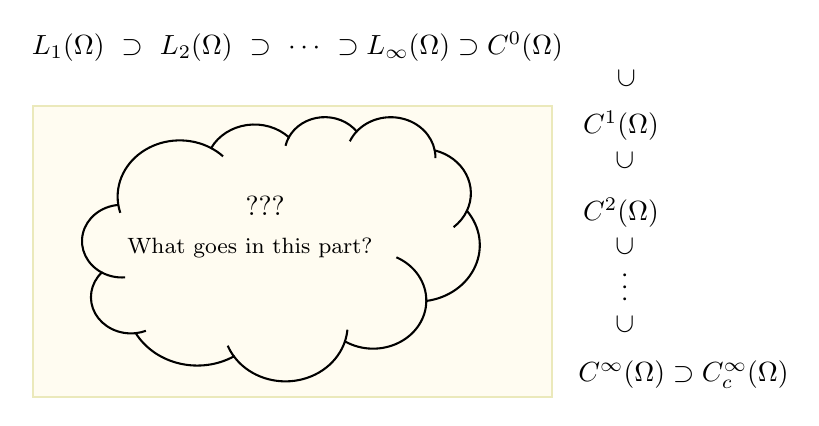
\begin{tikzpicture}[x=0.75pt,y=0.75pt,yscale=-1,xscale=1]
	%uncomment if require: \path (0,300); %set diagram left start at 0, and has height of 300
	
	%Shape: Rectangle [id:dp3131224415234657] 
	\draw  [color={rgb, 255:red, 235; green, 233; blue, 187 }  ,draw opacity=1 ][fill={rgb, 255:red, 255; green, 252; blue, 241 }  ,fill opacity=1 ] (120,90) -- (370,90) -- (370,230) -- (120,230) -- cycle ;
	%Shape: Cloud [id:dp6468787167291297] 
	\draw   (161.11,137.27) .. controls (159.56,127.01) and (164.63,116.84) .. (174.16,111.1) .. controls (183.69,105.35) and (196,105.03) .. (205.88,110.26) .. controls (209.38,104.29) and (215.79,100.18) .. (223.16,99.15) .. controls (230.54,98.12) and (238.01,100.31) .. (243.33,105.05) .. controls (246.31,99.64) and (252.16,96) .. (258.81,95.43) .. controls (265.46,94.86) and (271.96,97.44) .. (276.01,102.25) .. controls (281.4,96.51) and (289.97,94.1) .. (298.02,96.05) .. controls (306.06,98) and (312.13,103.96) .. (313.61,111.37) .. controls (320.21,113) and (325.71,117.14) .. (328.68,122.72) .. controls (331.66,128.3) and (331.81,134.78) .. (329.12,140.48) .. controls (335.62,148.14) and (337.14,158.34) .. (333.11,167.27) .. controls (329.09,176.21) and (320.12,182.55) .. (309.56,183.91) .. controls (309.49,192.3) and (304.41,200) .. (296.27,204.04) .. controls (288.14,208.08) and (278.23,207.83) .. (270.36,203.39) .. controls (267,213.43) and (257.57,220.83) .. (246.12,222.37) .. controls (234.68,223.91) and (223.28,219.33) .. (216.85,210.61) .. controls (208.97,214.91) and (199.51,216.15) .. (190.61,214.04) .. controls (181.71,211.94) and (174.12,206.67) .. (169.55,199.43) .. controls (161.5,200.28) and (153.71,196.51) .. (150.05,189.97) .. controls (146.4,183.44) and (147.65,175.54) .. (153.19,170.2) .. controls (146.01,166.37) and (142.34,158.78) .. (144.11,151.38) .. controls (145.87,143.98) and (152.66,138.45) .. (160.95,137.67) ; \draw   (153.19,170.2) .. controls (156.59,172.01) and (160.5,172.83) .. (164.42,172.55)(169.55,199.43) .. controls (171.23,199.25) and (172.88,198.87) .. (174.46,198.3)(216.85,210.61) .. controls (215.66,209) and (214.67,207.28) .. (213.89,205.48)(270.36,203.39) .. controls (270.97,201.55) and (271.36,199.67) .. (271.54,197.76)(309.56,183.91) .. controls (309.64,174.98) and (304.04,166.8) .. (295.16,162.89)(329.12,140.48) .. controls (327.68,143.52) and (325.48,146.22) .. (322.71,148.36)(313.61,111.37) .. controls (313.86,112.59) and (313.97,113.84) .. (313.95,115.09)(276.01,102.25) .. controls (274.67,103.68) and (273.57,105.28) .. (272.73,107)(243.33,105.05) .. controls (242.61,106.35) and (242.08,107.72) .. (241.74,109.15)(205.88,110.26) .. controls (207.97,111.37) and (209.91,112.71) .. (211.64,114.24)(161.11,137.27) .. controls (161.32,138.69) and (161.66,140.08) .. (162.11,141.45) ;
	
	% Text Node
	\draw (118,52.75) node [anchor=north west][inner sep=0.75pt]    {$L_{1}( \Omega ) \ \supset \ L_{2}( \Omega ) \ \supset \ \cdots \ \supset L_{\infty }( \Omega ) \supset C^{0}( \Omega )$};
	% Text Node
	\draw (411.27,70) node [anchor=north west][inner sep=0.75pt]  [rotate=-90]  {$\supset $};
	% Text Node
	\draw (383.67,90.73) node [anchor=north west][inner sep=0.75pt]    {$C^{1}( \Omega )$};
	% Text Node
	\draw (383.67,132.73) node [anchor=north west][inner sep=0.75pt]    {$C^{2}( \Omega )$};
	% Text Node
	\draw (410.6,109.33) node [anchor=north west][inner sep=0.75pt]  [rotate=-90]  {$\supset $};
	% Text Node
	\draw (381.33,211.07) node [anchor=north west][inner sep=0.75pt]    {$C^{\infty }( \Omega ) \supset C_{c}^{\infty }( \Omega )$};
	% Text Node
	\draw (410.6,151) node [anchor=north west][inner sep=0.75pt]  [rotate=-90]  {$\supset $};
	% Text Node
	\draw (409.27,168) node [anchor=north west][inner sep=0.75pt]  [rotate=-90]  {$\cdots $};
	% Text Node
	\draw (410.6,188.33) node [anchor=north west][inner sep=0.75pt]  [rotate=-90]  {$\supset $};
	% Text Node
	\draw (221,132) node [anchor=north west][inner sep=0.75pt]   [align=left] {???};
	% Text Node
	\draw (164,152) node [anchor=north west][inner sep=0.75pt]   [align=left] {{\footnotesize What goes in this part?}};
	
	
\end{tikzpicture}
\end{figure}